% sections/architecture.tex

\section{System Architecture}
\label{sec:architecture}

We formalize the routing problem and present the three-layer architecture that decomposes it into composable signal extraction, decision evaluation, and plugin execution---enabling a single framework to serve diverse deployment scenarios through configuration.

\subsection{Problem Formulation}

Let $\mathcal{M} = \{m_1, \ldots, m_K\}$ denote a set of $K$ available model backends, each characterized by capability profile, cost, and latency.
Each backend may be served by a different provider $p_k \in \mathcal{P}$ (e.g., local vLLM, OpenAI, Anthropic, Azure, Bedrock, Gemini), with provider-specific API protocols and authentication mechanisms.
A deployment may expose multiple endpoints $\mathcal{E} = \{e_1, \ldots, e_L\}$ with weighted load distribution across backends.

Given an incoming request $r$ (consisting of a message sequence, metadata, user identity, and headers), the routing problem is to:
\begin{enumerate}[leftmargin=*]
  \item Select a model $m^* \in \mathcal{M}$ that maximizes response quality while respecting cost and latency constraints;
  \item Apply deployment-specific safety and privacy transformations $\mathcal{T}(r)$ before and after model invocation;
  \item Route through the correct provider endpoint with appropriate authentication.
\end{enumerate}

Na\"ive approaches either fix $m^*$ statically or route based on a single dimension (e.g., estimated difficulty).
We argue that production routing requires reasoning over \emph{multiple orthogonal signal dimensions simultaneously}, with different \emph{policies} (safety thresholds, caching strategies, prompt augmentation, model pools) for different routing outcomes---and that these policies must be \emph{composable} to support diverse deployment scenarios without architectural changes.

\subsection{Composable Signal Orchestration}

The key architectural innovation is that the same signal extraction, decision evaluation, and plugin execution machinery can be \emph{composed differently} for different deployment scenarios:

\begin{definition}[Deployment Configuration]
A deployment configuration $\Gamma = (\mathcal{S}_\Gamma, \mathcal{D}_\Gamma, \Pi_\Gamma, \mathcal{E}_\Gamma)$ specifies which signal types $\mathcal{S}_\Gamma \subseteq \mathcal{S}$ are active, what decisions $\mathcal{D}_\Gamma$ are evaluated, which plugin chains $\Pi_\Gamma$ are attached, and which endpoints $\mathcal{E}_\Gamma$ are available.
\end{definition}

\noindent\textbf{Example configurations:}
\begin{itemize}[leftmargin=*]
  \item \emph{Privacy-regulated (healthcare)}: Active signals include domain, authz, and language. Decisions route sensitive queries to on-premise models only. Plugins enforce strict PII redaction with no caching.
  \item \emph{Cost-optimized (developer tool)}: Active signals include complexity, embedding, and keyword. Decisions cascade from cheap to expensive models. Plugins enable aggressive semantic caching.
  \item \emph{Multi-cloud enterprise}: Active signals include domain, modality, and authz. Decisions distribute across multiple provider endpoints using latency-aware model selection with weighted failover. Plugins inject provider-specific auth headers.
\end{itemize}

All three scenarios use the same architecture; only $\Gamma$ differs. This composability is the central design contribution.

\subsection{Three-Layer Architecture}

The architecture decomposes routing into three layers, each with a well-defined interface (\Cref{fig:architecture}):

\begin{figure*}[t]
  \centering
  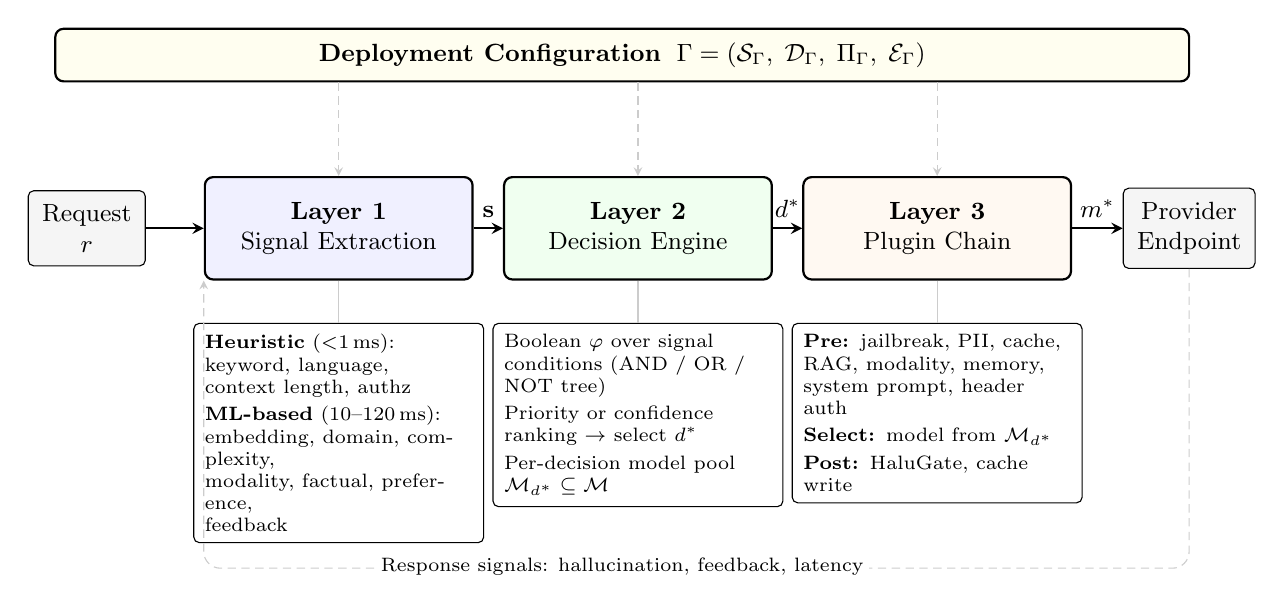
\begin{tikzpicture}[
    layer/.style={rectangle, draw, thick, rounded corners=3pt,
                  minimum height=1.3cm, minimum width=3.4cm, align=center,
                  inner sep=5pt, font=\small},
    io/.style={rectangle, draw, rounded corners=2pt, fill=black!4,
               font=\small, inner sep=5pt, align=center,
               minimum width=1.4cm},
    detail/.style={rectangle, draw, thin, rounded corners=2pt,
                   fill=white, font=\scriptsize, align=left,
                   text width=3.4cm, inner sep=4pt},
    arr/.style={->, >=stealth, thick},
    darr/.style={->, >=stealth, densely dashed, gray!40},
    lbl/.style={font=\small, above, midway},
  ]

  % Configuration bar
  \node[rectangle, draw, thick, rounded corners=3pt, fill=yellow!6,
        minimum width=14.4cm, inner sep=5pt, font=\small]
    (cfg) at (5.6, 3.0)
    {\textbf{Deployment Configuration}\;
     $\Gamma = (\mathcal{S}_\Gamma,\;
     \mathcal{D}_\Gamma,\;
     \Pi_\Gamma,\;
     \mathcal{E}_\Gamma)$};

  % Input
  \node[io] (req) at (-1.2, 0.8) {Request\\$r$};

  % Layer boxes
  \node[layer, fill=blue!6]   (L1) at (2.0,  0.8) {\textbf{Layer 1}\\Signal Extraction};
  \node[layer, fill=green!6]  (L2) at (5.8,  0.8) {\textbf{Layer 2}\\Decision Engine};
  \node[layer, fill=orange!5] (L3) at (9.6, 0.8) {\textbf{Layer 3}\\Plugin Chain};

  % Output
  \node[io] (out) at (12.8, 0.8) {Provider\\Endpoint};

  % Main flow arrows
  \draw[arr] (req)  -- (L1);
  \draw[arr] (L1)   -- node[lbl] {$\mathbf{s}$} (L2);
  \draw[arr] (L2)   -- node[lbl] {$d^*$} (L3);
  \draw[arr] (L3)   -- node[lbl] {$m^*$} (out);

  % Config arrows down
  \draw[darr] (cfg.south -| L1) -- (L1.north);
  \draw[darr] (cfg.south -| L2) -- (L2.north);
  \draw[darr] (cfg.south -| L3) -- (L3.north);

  % Detail boxes
  \node[detail, anchor=north] (d1) at (2.0, -0.4) {%
    \textbf{Heuristic} ({$<$}1\,ms):\\
    keyword, language,\\
    context length, authz\\[2pt]
    \textbf{ML-based} (10--120\,ms):\\
    embedding, domain, complexity,\\
    modality, factual, preference,\\
    feedback};

  \node[detail, anchor=north] (d2) at (5.8, -0.4) {%
    Boolean $\varphi$ over signal\\
    conditions (AND / OR / NOT tree)\\[2pt]
    Priority or confidence\\
    ranking $\to$ select $d^*$\\[2pt]
    Per-decision model pool\\
    $\mathcal{M}_{d^*} \subseteq \mathcal{M}$};

  \node[detail, anchor=north] (d3) at (9.6, -0.4) {%
    \textbf{Pre:} jailbreak, PII, cache,\\
    RAG, modality, memory,\\
    system prompt, header auth\\[2pt]
    \textbf{Select:} model from $\mathcal{M}_{d^*}$\\[2pt]
    \textbf{Post:} HaluGate, cache write};

  % Thin lines connecting layer boxes to detail boxes
  \draw[thin, gray!40] (L1.south) -- (d1.north);
  \draw[thin, gray!40] (L2.south) -- (d2.north);
  \draw[thin, gray!40] (L3.south) -- (d3.north);

  % Feedback loop
  \draw[darr, rounded corners=6pt]
    (out.south) -- ++(0,-3.8) -| (L1.south west);
  \node[font=\scriptsize, fill=white, inner sep=2pt]
    at (5.6, -3.5)
    {Response signals: hallucination, feedback, latency};

  \end{tikzpicture}
  \caption{Three-layer architecture with closed-loop feedback. A deployment configuration~$\Gamma$ selects which signals, decisions, and plugins are active. Layer~1 extracts a signal vector~$\mathbf{s}$ from the request. Layer~2 evaluates Boolean decision formulas to select~$d^*$. Layer~3 executes the per-decision plugin chain, selects a model from~$d^*$'s candidate set, and routes to the provider endpoint. Response-side signals feed back to enable adaptive routing.}
  \label{fig:architecture}
\end{figure*}

\textbf{Layer 1: Signal Extraction.}
The signal layer maps a request $r$ to a structured signal result $\mathbf{s}$, consisting of binary match indicators and real-valued confidences for each configured rule across eleven signal types.
Heuristic signals (keyword, language, context length, authorization) complete in sub-millisecond time.
ML-based signals (embedding similarity, domain classification, factual grounding, modality detection, complexity, preference, user feedback) require neural inference at 10--120\,ms.
Signals are evaluated in parallel, and only signal types referenced by at least one active decision are computed---a critical optimization for deployment configurations that use a subset of available signals.

\textbf{Layer 2: Decision Evaluation.}
The decision layer takes the signal result $\mathbf{s}$ and evaluates a set of decisions $\mathcal{D} = \{d_1, \ldots, d_M\}$, each defined as a Boolean formula over signal conditions.
The engine selects the best-matching decision $d^*$ using either priority-based or confidence-weighted ranking.
Each decision carries its own model candidate set $\mathcal{M}_{d^*} \subseteq \mathcal{M}$, enabling deployment-specific model pools (e.g., a privacy decision restricts candidates to on-premise models).

\textbf{Layer 3: Plugin Chain.}
Each decision $d^*$ carries a per-decision plugin configuration that defines:
(a)~\emph{pre-routing plugins} (jailbreak detection, PII filtering, semantic caching, RAG context injection, modality routing, memory retrieval, system prompt augmentation, header mutation for provider auth), executed before model invocation;
(b)~a \emph{semantic model selection algorithm} applied to $d^*$'s candidate model set $\mathcal{M}_{d^*}$ to find the best model cost-effectively;
(c)~\emph{post-routing plugins} (hallucination detection, cache updates), executed on the model response.

\subsection{Design Principles}

Four principles guide the architecture:

\textbf{Composability.}
Complex routing policies are expressed as compositions of simple primitives: Boolean combinations of signal conditions form decisions; sequences of typed plugins form execution chains; deployment scenarios are expressed as configuration profiles.
This avoids monolithic routing logic and enables the same system to serve fundamentally different deployment requirements.

\textbf{Orthogonality.}
Signals, decisions, and plugins are independent modules with a uniform interface boundary.
New signal types can be added by implementing a single evaluation function---the decision engine references signals solely by type and rule name, requiring no modification.
Likewise, new plugins and providers are registered independently.
The current eleven signal types are the built-in set; the framework is designed to be extended with domain-specific signals as deployment requirements evolve.

\textbf{Closed-loop adaptivity.}
The bidirectional signal flow described in \Cref{sec:signal_engine} enables the architecture to operate as a \emph{closed-loop control system}~\cite{astrom2008feedback}.
In control-theoretic terms, the signal--decision--plugin pipeline is the \emph{plant}, response-side signals (hallucination detection, user feedback, latency measurements) are the \emph{sensors}, and a policy adjustment mechanism is the \emph{controller} that updates decision parameters $\theta^{(t)}$ (priorities, model weights) based on observed response quality:
\begin{equation}
  \theta^{(t+1)} = \theta^{(t)} + \eta \,\nabla_\theta\, \mathbb{E}\bigl[Q\bigl(r,\, m^*(r;\theta^{(t)})\bigr)\bigr]
\end{equation}
where $Q(r, m^*)$ is a response quality metric and $\eta$ is a learning rate.
This formulation connects to the \emph{contextual bandit} framework~\cite{li2010contextual}: the signal vector $S(r)$ serves as the context, model selection is the action, and response quality is the reward.
Standard regret bounds from online learning theory~\cite{shalev2012online} guarantee that the cumulative routing quality of such an adaptive policy converges to that of the best fixed policy in hindsight at a rate of $O(\sqrt{T})$, providing formal performance guarantees for self-improving routing.

\textbf{Per-decision scoping.}
Safety thresholds, caching policies, model candidates, and auth mechanisms are scoped to individual decisions rather than applied globally.
A coding-focused decision can disable PII detection while a customer-support decision enforces strict filtering---using the same system configuration.

\textbf{Provider abstraction.}
The architecture abstracts over provider-specific protocols, authentication, and endpoint topologies.
Multi-endpoint routing with weighted distribution and failover is handled at the infrastructure layer, enabling decisions to reference models by capability rather than by provider-specific endpoint.
